\documentclass[border=10pt]{standalone}
\usepackage{pgfplots}
\usepackage{tikz}
\pgfplotsset{width=13cm,compat=1.8}

\begin{document}
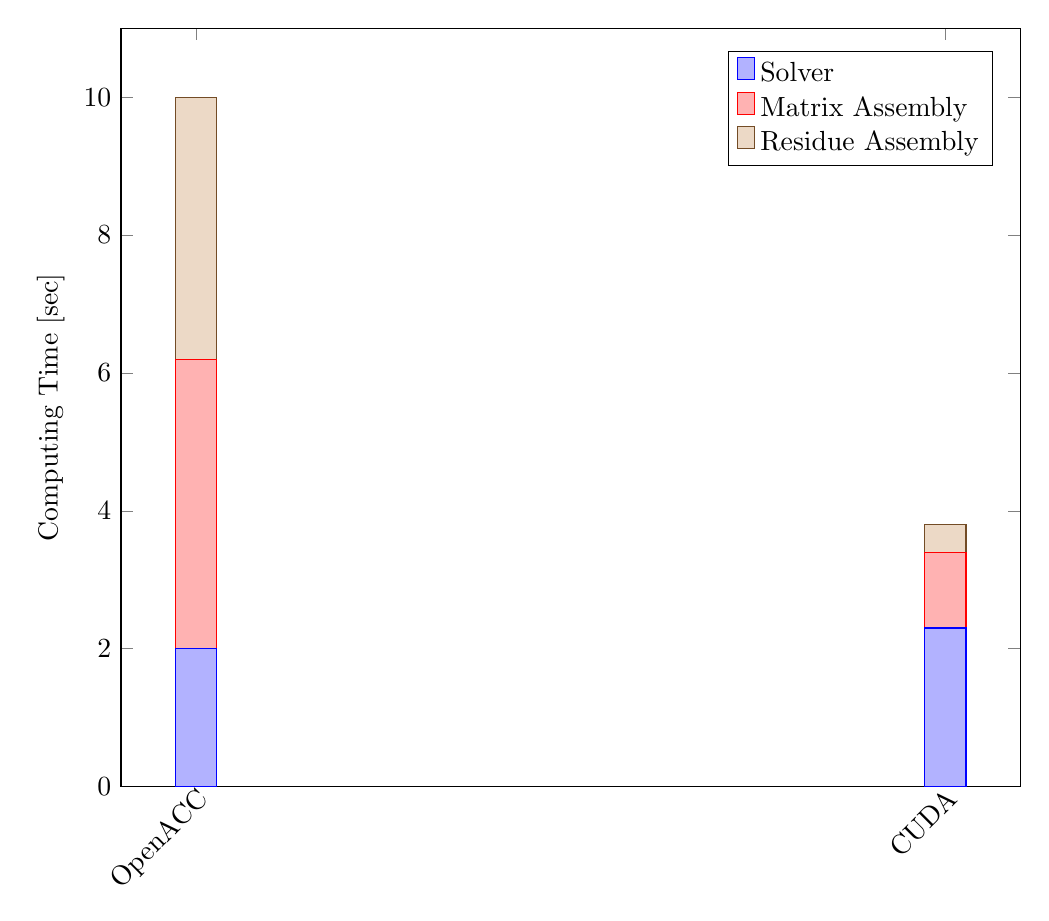
\begin{tikzpicture}[]
  \begin{axis}[scale=1.0,
      ybar stacked,
      bar width=15pt,
      %enlargelimits=0.15,
      ymin=0,
      ylabel={Computing Time [sec]},
      symbolic x coords={OpenACC, CUDA},
      x tick label style={rotate=45, anchor=north east, inner sep=0mm},
      xtick=data,
      legend pos=north east,
      legend cell align={left},
      legend style={fill=white,anchor=north east}
    ]
    \addplot+[ybar] plot coordinates {
      (OpenACC,2) 
      (CUDA,2.3)
    }; % sol cpu
    \addplot+[ybar] plot coordinates {
      (OpenACC,4.2)
      (CUDA,1.1)
    }; % mat
    \addplot+[ybar] plot coordinates {
      (OpenACC,3.8)
      (CUDA,0.4)
    }; % res cpu
    %\addplot+[ybar] plot coordinates {
    %  (Wilkes-2 CPU,13.5)   (Wilkes-2 GPU,14.45)
    %  (POWER9 CPU,14.4)  (POWER9 GPU,16.1)
    %  (Cirrus CPU,21.8)      (Cirrus GPU,22.8)
    %}; % other (cpu)

    \legend{Solver, Matrix Assembly, Residue Assembly, Others};
  \end{axis}
\end{tikzpicture}

% CPU
% ell_solve_cgpd                   92.9
% assembly_mat                     18.2
% assembly_rhs                     7.9
% other                            8.1
% total                            127

% OpenACC
% ell_solve_cgpd_acc               2.0
% assembly_mat_acc                 4.2
% assembly_rhs_acc                 3.8
% other                            6.1
% total                            16.1

% CUDA
% ell_solve_cgpd_cuda              2.3
% assembly_mat_cuda                1.1
% assembly_rhs_cuda                0.4
% other                            8.4
% total                            12.2

\end{document}
